%=====================================================================
%  UPRM Weight Gym Operations and Member-Access Platform
%  CIIC 4151 Senior Design Project
%  Overleaf-ready LaTeX source (compile with pdfLaTeX)
%
%  Progress report: built from the proposal (docs/capstone_proposal/v0), one file per section in sections/.
%=====================================================================
\documentclass[11pt,letterpaper]{article}

%---------------------------- Encoding ------------------------------
\usepackage[utf8]{inputenc}     % accented characters: Mayagüez, José, Miłosz
\usepackage[T1]{fontenc}
\usepackage[english]{babel}
\IfFileExists{lmodern.sty}{\usepackage{lmodern}}{} % optional nicer font

%---------------------------- Layout --------------------------------
\usepackage[margin=1in]{geometry}
\usepackage{setspace}
\usepackage{parskip}
\usepackage{fancyhdr}
\usepackage{titlesec}

%---------------------------- Tables --------------------------------
\usepackage{array}
\usepackage{tabularx}
\usepackage{longtable}
\usepackage{booktabs}
\usepackage{ragged2e}

%---------------------------- Lists / Figures -----------------------
\usepackage{enumitem}
\usepackage{graphicx}
\usepackage{xcolor}
% Open items that wait on a decision or on code. List them with: grep -rn "\\pending" sections
\newcommand{\pending}[1]{\textcolor{red}{\textbf{[PENDING:} #1\textbf{]}}}
% Text that changed after the proposal review or is new in this report. List it with: grep -rn "\\revised" sections
% Delivery versions from one source. Review look (default): \showchangestrue \reviewroundtrue.
% Changes in blue: \showchangestrue \reviewroundfalse. Clean black: \showchangesfalse.
\newif\ifshowchanges \showchangestrue
\newif\ifreviewround \reviewroundtrue
\InputIfFileExists{version.tex}{}{} % CI writes the delivery flags here
\ifshowchanges
  \DeclareRobustCommand{\revised}[1]{{\color{blue!70!black}#1}}
  \ifreviewround
    % Text added or rewritten in round 3 of the review. List it with: grep -rn "\roundthree" sections
    \DeclareRobustCommand{\roundthree}[1]{{\color{violet!80!black}#1}}
  \else
    \DeclareRobustCommand{\roundthree}[1]{{\color{blue!70!black}#1}}
  \fi
\else
  \DeclareRobustCommand{\revised}[1]{#1}
  \DeclareRobustCommand{\roundthree}[1]{#1}
\fi
\usepackage{caption}

%---------------------------- Links ---------------------------------
\usepackage[hidelinks]{hyperref}
\usepackage{url}
\urlstyle{same}
\pdfstringdefDisableCommands{\renewcommand{\revised}[1]{#1}\renewcommand{\roundthree}[1]{#1}} % keep bookmarks plain
\IfFileExists{xurl.sty}{\usepackage{xurl}}{} % break long URLs anywhere

%------------------- Global formatting choices ----------------------
% Sections are numbered with Roman numerals (I. INTRODUCTION ... VII. ...)
\renewcommand{\thesection}{\Roman{section}}
\titleformat{\section}{\normalfont\large\bfseries}{\thesection.}{0.6em}{\MakeUppercase}
\titleformat{\subsection}{\normalfont\normalsize\bfseries}{}{0em}{}
\titleformat{\subsubsection}{\normalfont\normalsize\itshape}{}{0em}{}
\setcounter{secnumdepth}{1}   % only top-level sections are numbered

% "Figure 1." instead of "Figure 1:"
\captionsetup{labelsep=period,font=small,labelfont=bf}

% Ragged-right, fixed-width column type used by all tables
\newcolumntype{L}[1]{>{\RaggedRight\arraybackslash}p{#1}}

\pagestyle{fancy}
\fancyhf{}
\fancyhead[L]{\small UPRM Weight Gym Operations and Member-Access Platform}
\fancyhead[R]{\small\thepage}
\renewcommand{\headrulewidth}{0.4pt}

\setlength{\emergencystretch}{1.5em}   % avoid overfull lines
\setlist[itemize]{leftmargin=1.5em,itemsep=2pt,topsep=3pt}
\setlist[enumerate]{leftmargin=2em,itemsep=2pt,topsep=3pt}

%=====================================================================
\begin{document}

%--------------------------- TITLE PAGE ------------------------------
\begin{titlepage}
\thispagestyle{empty}
\centering
\vspace*{3.5cm}

{\LARGE\bfseries UPRM Weight Gym Operations and\\[0.3cm] Member-Access Platform\par}

\vspace{4cm}

{\large CIIC 4151 Senior Design Project\par}
\vspace{0.6cm}
{\large Carlos J. Pepin Delgado\par}
{\large Pierre G. Vales Torres\par}
{\large Viviana V. Ramos Vivoni\par}

\vspace{2cm}

{\large Advisor: Fernando Torre\par}
{\large Prof. Wilson Rivera\par}
\vspace{0.4cm}
{\large Department of Computer Science and Engineering\par}
{\large University of Puerto Rico at Mayaguez Campus\par}
\vspace{0.4cm}
{\large Progress Report\par}
\vspace{0.4cm}
{\large November 10th, 2026\par}

\vfill
\end{titlepage}

%=====================================================================
\section*{Response to Proposal Reviews}
\addcontentsline{toc}{section}{Response to Proposal Reviews}
%=====================================================================

The proposal received four comments. Each row below says what the team changed and where to find it in this report.

\begin{center}
\small
\begin{longtable}{L{3.3cm} L{6.4cm} L{3.7cm}}
\toprule
\textbf{Comment} & \textbf{What we changed} & \textbf{Where in this report} \\
\midrule
\endfirsthead
\toprule
\textbf{Comment} & \textbf{What we changed} & \textbf{Where in this report} \\
\midrule
\endhead
\bottomrule
\endlastfoot
\textbf{5(b) Diagrams.} ``I would have also appreciated some UI sketches or wireframes.'' & Listed the 40 screens by role with their states and drew seven navigation maps. Viviana drew the wireframes in Figma, split into six issues; the Check In, sign-in, and Staff sets are approved. \pending{wireframe figures exported from Figma, Viviana, issues \#40 to \#45} & Technical Approach, User Interface Design \\
\addlinespace
\textbf{5(d) Constraints.} Missing requirements from the Capstone guidelines, such as accessibility. & Added accessibility (WCAG 2.2 level AA) as a constraint with its checks: axe-core in CI, lint rules, and a manual checklist. Added the CTI VM, polling, and mail dependency, and removed refund and cancellation text. & Technical Approach, Engineering Constraints and Verification \\
\addlinespace
\textbf{5(e) Standards.} Missing authentication standards. & Added NIST SP 800-63B-4 and OWASP ASVS 5.0.0 with the controls we apply: password rules, attempt limits, sessions, and role checks. Individual accounts with roles replace the shared gym account. & Technical Approach, Engineering Standards; Identity, Authorization, and Session Model \\
\addlinespace
\textbf{5(e) Architecture.} System Architecture was expected in this section or the next. & Added a System Architecture subsection with the components, the Check In request path, and the deployment on a CTI VM. & Technical Approach, System Architecture \\
\addlinespace
\textbf{6(d) Testing plan.} Missing acceptance and stress testing. & Added an acceptance test with gym staff and real users and a load test with k6 for simultaneous Check Ins. & Project Plan, Testing Plan; Preliminary Results, Testing Plan Execution \\
\addlinespace
\textbf{Changes since the proposal.} & Moved to Laravel, PostgreSQL, and docker-compose on a CTI VM, with polling instead of real-time updates, own accounts, paid memberships read from the store's API, and a revised phase schedule. & Solution Approach, Changes since the Proposal \\
\end{longtable}
\end{center}


%=====================================================================

\section{Introduction}
%=====================================================================

The Gimnasio de Pesas at the University of Puerto Rico at Mayagüez (UPRM), located at the Natatorio Complex, relies on manual registration and access-verification steps and uses paper-based records for registration. Staff must confirm whether a person is authorized to enter through a paid membership or athlete authorization. Because these authorization sources come from separate processes, users may need to provide proof of payment while staff check different records before granting access. The records also do not automatically provide an active-user count or facility-use metrics such as peak usage periods, occupancy patterns, or differences among user groups.

A stakeholder assessment on September 11, 2026, with the Director of UPRM's Department of Athletic Activities, José F. Estévez Pérez, and two Athletic Activities staff members who work alongside the Director and are familiar with the current operational processes, confirmed these concerns. They reported reliability problems with manual access verification, said that facility-use metrics matter for administrative decisions and for students, and said users need to hear about schedule changes, temporary closures, maintenance, and other operational updates. The Director estimated that about 150 people use the Weight Gym each day, so staff repeat these verification and registration steps about 150 times a day. At the same time, some information needed for access verification already exists digitally. UPRM uses WooCommerce to manage gym membership payments, and a completed order indicates a successful payment. However, staff still perform payment verification and check-in manually, while the process does not automatically use check-in records to calculate occupancy or generate utilization metrics.

Since the proposal, the team has worked with two more stakeholders. On October 22, 2026, three team members met the contact at UPRM's Centro de Tecnologías de Información (CTI), the office that will host the application. CTI said it uses Laravel and suggests it to other projects, left the database and containers to the team, and said that the project owner, the gym director, files the virtual machine, domain, and VPN requests and answers for the accounts he authorizes. CTI also said it has no staff to maintain the application after December, so the owner must plan who looks after it. The minutes are in the project repository (\texttt{docs/meetings/2026-10-22-cti-minuta.md}). On November 4, 2026, the team meets the gym director to settle the open questions about the athlete roster, Check In rules, and staff accounts: \pending{director meeting outcomes}. This report shows what those meetings changed, what the team has built, and what remains before the final report on December 11.


%=====================================================================

\section{Problem Statement}
%=====================================================================

This project addresses the divided access and facility-use process at the Gimnasio de Pesas. Authorization depends on separate sources (WooCommerce for paid memberships and administrative records for athletes) that staff must verify manually, and check-ins do not produce a centralized count of active users or consistent utilization metrics.

This is a relevant problem because the manual process is outdated and needed updating, and stakeholder discussions with UPRM Athletic Activities Director José F. Estévez confirmed the need and supported its selection as a Capstone project. It requires the design, implementation, and testing of an integrated software system. The software must determine authorization from multiple eligibility sources, enforce permissions for users, staff, and administrators, maintain active facility sessions, and transform recorded facility use into consistent utilization metrics. It also presents engineering challenges such as integrating with WooCommerce; keeping sessions and occupancy consistent under simultaneous requests; protecting sensitive user information; and handling imprecise indoor location and loss of connectivity. These behaviors can be evaluated through measurable software requirements and acceptance tests.


The target domain is university athletic-facility access and utilization operations. This domain covers the operational processes used to determine who is authorized to use a facility, register facility entry and use, maintain current operating schedules and temporary operational changes, and collect facility-use records that can support estimated occupancy and the identification of utilization patterns. This project belongs to that domain because it addresses how an athletic facility controls access, records facility use, communicates current operational information, and uses those records to support daily operations and administrative decision-making. For the current core scope, the project addresses these processes for the Gimnasio de Pesas located in the UPRM Natatorio Complex. Out of scope are payment processing, which remains in the existing WooCommerce process; access workflows for other facilities, including the pool, which have separate rules and authorization needs; medical-record management, since only safety information UPRM Athletic Activities deems necessary is kept; and capacity-based admission control, which requires an official UPRM capacity policy.

The intended users of the system fall into two groups. Facility users are authorized individuals who use the Gimnasio de Pesas through a paid membership or athlete authorization. Operational users include facility staff, including student workers assigned to reception or check-in duties, who monitor or assist with facility entry, and administrators who manage authorization records, athlete rosters, schedules, access rules, and utilization information. The principal stakeholders include the Departamento de Actividades Atléticas, because it owns the operational need being addressed; Prof. José F. Estévez, because he represents the client in project decisions; facility staff and administrators, because the system affects the processes they use to verify access and manage the facility; and authorized facility users, because the system affects how their access and facility use are recorded and communicated.

The proposed innovation is an integrated access and facility-use management platform for the Gimnasio de Pesas. It connects institutional login, access authorization (paid semester membership or preapproved athlete roster), location-validated check-in, active sessions, estimated occupancy, operating schedules, and utilization analytics in one workflow. It leaves the WooCommerce payment process in place and uses completed membership orders to determine paid access. A successful check-in creates a facility-use record that supports current operations and later analysis.

%=====================================================================

\section{Project Objectives}
%=====================================================================

The five objectives and their metrics are unchanged. Three acceptance criteria changed after design decisions (Objectives 3, 4, and 5), and the deadlines now follow the six phases of the project plan (issue \#50; Midterm report on November 9, Final report on December 11). The status column is traced to the issue tracker on November 4, 2026.

\begin{center}
\footnotesize
\setlength{\tabcolsep}{4pt}
\begin{longtable}{L{2.6cm} L{3.3cm} L{4.6cm} L{2.0cm} L{2.2cm}}
\toprule
\textbf{Objective} & \textbf{Metric} & \textbf{Acceptance Criteria} & \textbf{Target date} & \textbf{Status} \\
\midrule
\endfirsthead
\toprule
\textbf{Objective} & \textbf{Metric} & \textbf{Acceptance Criteria} & \textbf{Target date} & \textbf{Status} \\
\midrule
\endhead
\bottomrule
\endlastfoot

1. Consolidate user identity and facility-access authorization into one correct access decision.
&
Percentage of authorization cases correctly approved or denied using a controlled dataset with valid and expired paid memberships, valid and invalid athlete authorizations, missing authorization, and unmatched user records.
&
Every defined authorization case must return the expected decision. Users with valid authorization must be approved, while users without valid authorization must be denied.
&
Nov 8 for the access decision on controlled data (Phase 3); Nov 22 for registration and import (Phase 4)
&
In progress. Rules, flows, and data model done; schema (\#13) assigned, not merged. \\
\addlinespace
\midrule
\addlinespace

2. Implement a user-initiated check-in process that creates and manages a valid facility session from check-in through automatic expiration.
&
Percentage of defined check-in and session scenarios that reach the expected state, including location validation, successful and rejected check-ins, session creation, Gym ID generation, duplicate attempts, and 60-minute expiration.
&
Every valid check-in must create exactly one active session and one current Gym ID. Invalid attempts must create no session, duplicate attempts must follow the defined session rule, and each active session must stop counting as active after its 60-minute expiration.
&
Nov 8 (Phase 3: Check In)
&
In progress. Design done; location boundary not yet measured at the gym (\#12); Check In code (\#17) not started. \\
\addlinespace
\midrule
\addlinespace

3. Maintain a consistent active-session state and use it to provide estimated facility occupancy across the platform.
&
Difference between the estimated occupancy reported by the system and the expected number of active sessions after check-ins, expirations, Staff corrections, and concurrent session events.
&
The reported estimated occupancy must match the number of active session records in every tested state. User, Staff, and Administrator screens must show the same value once each screen has refreshed; screens poll the server every 20 to 30 seconds, so the test compares values after each refresh.
&
Nov 8 (Phase 3: Check In)
&
In progress. Design done; occupancy code (\#18) not started. \\
\addlinespace
\midrule
\addlinespace

4. Provide Staff and Administrators with role-controlled tools to supervise facility use and maintain operational information.
&
Percentage of role-permission checks and administrative tasks that produce the expected result according to the final User, Staff, and Administrator permission matrix.
&
Every tested action must be allowed or denied according to the assigned role. Staff and Administrators sign in with individual accounts, and an Administrator invites each person by email and assigns the role. Staff must be able to perform the defined monitoring and session-correction tasks, while Administrators must be able to manage athlete authorizations, schedules, closures, and Staff accounts.
&
Nov 29 (Phase 5: Staff and administration)
&
Planned. Design done; build work not started. \\
\addlinespace
\midrule
\addlinespace

5. Transform recorded facility-use data into utilization metrics that support operational decision-making.
&
Percentage of finalized utilization metrics that match their known expected values when calculated from controlled historical check-in and session datasets.
&
Every finalized metric must match its expected value in the controlled datasets, including utilization by time period, periods of higher and lower use, estimated occupancy trends and approved summary values, and utilization by authorization type. Analytics are open to every signed-in role and show aggregated counts only, with no names.
&
Nov 29 (Phase 5: Staff and administration)
&
Planned. Design done; analytics (\#29) not started. \\
\end{longtable}
\end{center}

No objective is Done: the repository holds the project skeleton and its continuous-integration tests, but no product behavior is implemented yet. \emph{In progress} means the requirements and design for the objective are complete and either its phase has started (Phase 3 began on November 2) or its first dependency, the database (\#13), is assigned. \emph{Planned} means its phase has not started. All objectives are verified together in the acceptance test with the gym (\#32) before the final report on December 11. The controlled datasets and test evidence for Objectives 1 to 3 are tracked in issue \#81.

%=====================================================================

\section{Solution Approach}
%=====================================================================

The solution is a Progressive Web Application (PWA) for the UPRM Weight Gym located in the Natatorio Complex. The platform brings together user accounts, semester-based authorization, Check In, current Gym ID verification, estimated occupancy, athlete management, facility information, membership records, and utilization analytics. The PWA is intended primarily for use from a user's phone while remaining accessible through a web browser. The system supports three roles: User, Staff, and Administrator.

\subsection{Changes since the Proposal}

Design review, the CTI meeting, and team decisions changed the proposal in the ways below. Status follows the project's decision log: Decided means the team agreed, Proposed means it needs confirmation, Pending means information is missing.

\begin{center}
\footnotesize
\setlength{\tabcolsep}{4pt}
\begin{longtable}{L{4.7cm} L{5.6cm} L{4.7cm}}
\toprule
\textbf{Change} & \textbf{Reason} & \textbf{Status} \\
\midrule
\endfirsthead
\toprule
\textbf{Change} & \textbf{Reason} & \textbf{Status} \\
\midrule
\endhead
\bottomrule
\endlastfoot

Stack: Laravel and PostgreSQL in \texttt{docker-compose} replace Supabase and Vercel.
&
CTI can host it in December, no external service holds student data, and the cost stays lowest.
&
Decided. Skeleton merged (\#46 to \#48). \pending{professor: approval of the stack change (question P-03), not answered yet} \\
\addlinespace

Hosting: development on each member's PC; production on a CTI virtual machine with a UPRM subdomain; VPN for the team.
&
What is tested is what runs in December. CTI said the project owner files the requests.
&
Decided. Requests being prepared (\#64). The team asks for 2 processors, 8 GB of memory, a 60 GB disk, and a 40 GB second disk for backups. \\
\addlinespace

Updates: the screen polls every 20 to 30 seconds instead of using real-time channels.
&
Occupancy changes only on a Check In or an expiration. Server-sent events failed through the test tunnel.
&
Decided. Live updates only if CTI allows them and time remains. \\
\addlinespace

Accounts: own accounts, no institutional login or SAML.
&
Some paid members have no UPRM email. CTI said SAML is only needed for external authentication.
&
Decided (no SAML). Built: sign-in, one device per User, password reset, and account deletion (\#15). \\
\addlinespace

Staff and Administrators: individual accounts with roles, invited by email by an Administrator. The shared gym account, the PIN, and the paper recovery code are removed. An install command creates the first Administrator.
&
The audit log can name the person who acted, as CTI suggested. It also matches the proposal's original User, Staff, and Administrator roles.
&
Decided on November 4, after the meeting with the department. The Administrators are the two department secretaries and the director. Built (\#16, \#84). \\
\addlinespace

Registration: one field for a number. A 9-digit student number is looked up in the athlete roster; anything else is looked up as an Authorization Number. The account email of a paid member is the WooCommerce payment email. Athletes open a link sent to their roster email.
&
Some members have no institutional email. A student number is not secret, so a link proves control of the roster email. Number lookups have rate limits.
&
Decided. Paid member backend merged, screens being finished (\#22). Athlete registration (\#23) is planned for the Final report milestone. \\
\addlinespace

Renewal and type change happen inside the existing account. A visit stays open until Staff check the person out and closes by itself 2 hours after Check In; a closure or the end of the term ends every open visit. Staff apply 60 minutes as a guide when the gym is full. Before and during an athletes-only period, every User sees a notice with its start time; during it only athletes can Check In, and it never cuts a visit.
&
One account and one history per person. Occupancy needs one counting rule.
&
Decided on November 4. Check In and automatic closes built (\#17, \#85); the Staff check-out screen is part of \#26. \\
\addlinespace

Paid memberships come from the WooCommerce REST API with a read-only key, not from an uploaded export. Only completed orders give access; an order that later becomes cancelled or refunded loses it. Refunds happen in the UPR Payment Gateway, outside the store, so an Administrator revokes that access by hand with a reason.
&
A test read of all 84 store orders on November 4 worked with a read-only key, and the sync saves the Administrator a manual step.
&
Decided on November 4. The sync is planned for the Final report milestone (\#25). The sync waits on CTI for outgoing HTTPS from the VM to the store (M-12). \pending{CTI: answer on outgoing HTTPS from the VM to the store, asked as question 20 in Discussion \#78 and waiting} \\
\addlinespace

Safety records reduced to waiver acceptance with an emergency contact. No address, documents, or medical warnings. Each acceptance stores the version of the text the person accepted.
&
Least sensitive data that covers an emergency. The version shows what each person agreed to after the text changes.
&
Decided. Until the department sends the official text, registration shows a draft in Spanish and English with its own version. A drawn signature is planned for the Final report (\#102). \\
\addlinespace

Analytics open to every signed-in role, aggregated counts only.
&
Counts hold no personal data, and users can plan when to go.
&
Decided. \\
\addlinespace

Security rules: a growing wait after 10 failed sign-ins; no inactivity timeout for Users, while a Staff sign-in ends after 2 idle hours and an Administrator sign-in after 20 minutes; passwords of at least 10 characters checked against known breaches; account deletion without an active authorization; audit log with account, time, IP address, and before and after values.
&
A timeout could sign a user out between Check In and the front desk. Less personal data is kept, and analytics keep working.
&
Decided and built (\#15, \#16). The 10-character minimum is below the 15 that NIST SP 800-63B-4 asks for in some cases; the deviation is documented. \\
\addlinespace

Manual grant and revoke: Administrators grant or revoke an authorization with a logged reason, and can add an Authorization Number missing from the store data, valid for the current term.
&
Fixes order errors and refunds, and a paid member whose order the sync missed can still register.
&
Decided. Planned for the Final report (\#27). \\
\addlinespace

Check In location: in production the boundary is at most 50 meters from the gym.
&
Indoor accuracy varies; a phone test gave 19 m at home.
&
Built: the production app refuses to start with a boundary farther than 50 m (\#17). Measuring the boundary at the gym moves to the Final report (\#12). \\
\addlinespace

Scope: all five objectives are committed; the roster tool and the Install button move to the MVP. Administrators enter the athlete roster by hand. Real WooCommerce data is used only to test the integration.
&
Objectives 4 and 5 test items the proposal called Secondary. The department keeps the athlete lists only in Word. Less student data on team computers.
&
Decided. Install button and offline support built (\#14). \\
\addlinespace

Data kept 5 years: photos, waivers, emergency contacts, visits, and the audit log. A replaced photo is deleted when the new one arrives. Daily totals with no personal data are kept for good. After December, the two department secretaries look after the system.
&
The department wants to compare years, and CTI has no staff to maintain the application.
&
Decided on November 4 and 5. Deleting old data is planned for the Final report (\#71). \\
\addlinespace

Operations CTI expects: mail through the CTI gateway, backups with a tested restore, a disaster plan, an install script, an audit log nobody can edit.
&
CTI asks every student project for these. CTI did not say they are conditions for the VM.
&
Backups decided: a copy every two weeks on a second disk of the same VM, keeping the 2 most recent. The team plans Rocky Linux 10 on the server, because CTI is moving to it. Issues \#65 to \#69 planned for the Final report. \pending{CTI: authorize the VM on its mail gateway and confirm Rocky Linux 10 and the second disk; Carlos asks in \#63 and \#64} \\
\addlinespace

Plan: six phases with dates replace the eleven sprints; final date December 11.
&
Issues of about one person-week each, grouped into phases with dates (issue \#50).
&
In use. On November 8, Midterm milestone: 36 issues closed, 15 open. Final milestone: 1 closed, 30 open. \\
\end{longtable}
\end{center}

\subsection{Accounts and Authorization}

Users Create an Account or Sign In to one persistent account across semesters. Authorization is separate: a person can move between paid-member and athlete access without losing their account or Check In history. A current photograph is required at registration and each semester renewal; users cannot freely replace it during an active authorization period because it appears on the Gym ID. To reduce account sharing, a User can stay signed in on only one device; signing in on another device ends the previous session.

\textbf{Paid members.} UPRM continues to process semester purchases through WooCommerce. The user types the Authorization Number from the payment receipt, which the system checks against the paid orders it reads from the store, then creates a password, supplies a photograph, and accepts the waiver. Only identity and authorization fields (name, email, whether the buyer is a student or an employee, and membership details) are copied; billing, address, phone, and the order's student number are not. On expiration, the account remains, Check In is disabled, and the PWA shows an expired status and Renew option.

\textbf{Athletes.} A preapproved athlete types a 9-digit student number in the same field. If it matches the roster that Administrators enter by hand, the system sends a link to the institutional email on the roster record; the athlete opens it, creates a password, and supplies a photograph. No purchase or Authorization Number is required. Each roster record can be claimed by only one account. The account is created only after the athlete opens that link, and athlete registration (\#23) is planned for the Final report milestone.

\textbf{Staff and Administrators.} Each person has an individual account. The Administrators are the two department secretaries and the department director. An Administrator invites a person by email, assigns the Staff or Administrator role, and deactivates the account when the person leaves; an install command creates the first Administrator. There is no shared gym account and no PIN: Administrator actions need the Administrator role. Every sensitive action is written to an audit log that names the person, time, and IP address.

\subsection{Check In, Gym ID, and Occupancy}

Normal Check In verifies current authorization and device location against the Weight Gym boundary, then atomically prevents overlapping sessions and creates one facility session. The session stays open until Staff check the person out at the desk. A session nobody closes ends by itself 2 hours after Check In, and a closure or the end of the term ends every open session. A person may come back the same day: each entry after a check-out is a new visit, and stepping out briefly stays in the same session. The 60 minutes are a guide Staff apply when the gym is full; the app does not enforce them. Location is a Check In condition, not proof of physical presence; users are not tracked continuously. Authorized Staff may correct a session. The Gym ID displays name, photograph, authorization, the Check In time, and the time elapsed since then, with no countdown; Staff verifies these against backend session data rather than the display alone.

If an authorized user lacks a smartphone while physically present, Staff locates the account using an approved identification method, checks the current photograph and active authorization against backend records, and creates the same kind of session. This Staff-assisted Check In records the Staff actor and timestamp as an exception; it cannot bypass authorization or create a second active session.

Estimated occupancy equals the count of open sessions and updates after Check Ins, check-outs, automatic closes, or Staff corrections; each screen polls the server every 20 to 30 seconds. Users, Staff, and Administrators see the same estimate; people who leave without a check-out stay counted until the automatic close, so it is not a physical headcount.

\subsection{Operations and Facility Information}

Staff view active sessions, Check In times, authorization, and Gym IDs, assist with approved Check In exceptions, and make permitted session corrections. Administrators maintain the athlete roster and authorizations, Staff accounts, schedules, special hours, closures, and facility information. Utilization analytics are open to every signed-in role, as aggregated counts without names. Users see schedules and closures, gym rules, towel and footwear requirements (including Crocs and flip-flop restrictions), available machines, and approved equipment-use instructions now often communicated physically or verbally. Stakeholders also identified possible QR-based equipment instructions; these remain Stretch functionality.

To reduce reliance on physical membership records, the system stores a liability-waiver acceptance, with the version of the text accepted, and an emergency contact (name and phone), and nothing more. From Check In and session records, every signed-in role can review visits by hour, day, week, and month; high- and low-use periods; estimated occupancy over time; average and maximum occupancy summaries; and use by paid members versus athletes. These measures support staffing, scheduling, and facility planning.

\subsection{Gap with Existing Solutions}

UPRM Athletic Activities already maintains relevant information digitally, but the current Weight Gym workflow remains fragmented. Paid memberships are processed through WooCommerce, athlete authorization is maintained separately, and manual facility registration does not automatically produce active-session, estimated-occupancy, or utilization information.

\begin{center}
\small
\begin{tabularx}{0.98\textwidth}{L{3.2cm} L{2.5cm} L{2.5cm} L{2.5cm} X}
\toprule
\textbf{Capability} &
\textbf{Current UPRM} &
\textbf{GymMaster [1]} &
\textbf{TeamUp [2]} &
\textbf{Proposed Platform} \\
\midrule

Member/mobile account
&
No integrated Weight Gym account workflow
&
Supported
&
Supported
&
Persistent account across semesters \\

\addlinespace

Digital Check In
&
Manual registration
&
Supported
&
Supported
&
Location-validated Check In linked to a facility session \\

\addlinespace

Existing WooCommerce process
&
Used for paid memberships but separate from Check In
&
Not UPRM-specific
&
Not UPRM-specific
&
Preserved and integrated as the paid-authorization source \\

\addlinespace

Paid-member and athlete authorization
&
Separate processes
&
Not UPRM-specific
&
Not UPRM-specific
&
Combined in one Weight Gym authorization workflow \\

\bottomrule
\end{tabularx}
\end{center}

Member applications and digital Check In are common features of commercial gym software. GymMaster provides member-app and access-control capabilities [1], while TeamUp provides membership-linked access control, customer Check In, and form and waiver capabilities [2]. The proposed platform does not claim these individual capabilities as new. Its specific contribution is integrating them around UPRM's existing WooCommerce payment process, Administrator-managed athlete authorization, facility sessions, estimated occupancy, and operational requirements. ``Not UPRM-specific'' does not mean that a commercial platform lacks a comparable feature; it means that the feature is not designed around the institutional workflow addressed by this project.

\subsection{Value Proposition}

The platform connects UPRM's existing WooCommerce process and athlete authorization to one facility workflow, keeps each person's identity across semesters, and turns Check Ins into current sessions, occupancy estimates, and utilization data. It also puts access status, Gym ID, schedules, rules, equipment information, and approved membership records in one PWA.

\subsection{Scope Prioritization}

The team committed to all five objectives. The MVP is built and validated first; Secondary features follow in the same semester and are also committed. Stretch features follow only if committed work is complete and tested, or remain future work.

\begin{center}
\small
\begin{tabularx}{0.95\textwidth}{L{2.4cm} X}
\toprule
\textbf{Scope} & \textbf{Capabilities} \\
\midrule
MVP & Persistent accounts; paid-member and athlete authorization; paid memberships read from the WooCommerce API; Administrator roster tool; location-validated Check In; one open session per User, closed by Staff check-out or after 2 hours; current Gym ID; estimated occupancy; individual Staff and Administrator accounts with basic Staff verification and correction; Install button. \\
\addlinespace
Secondary (committed) & Full role permissions; schedules, closures, and notices; rules and equipment information; waiver acceptance and emergency contact; utilization analytics open to every signed-in role; audit log screen. \\
\addlinespace
Stretch / Future & Equipment QR shortcuts; capacity-based admission after UPRM sets an official policy; Natatorio or other facility expansion; predictive occupancy after enough history exists. \\
\bottomrule
\end{tabularx}
\end{center}

\subsection{Benefits and Limitations}

\begin{center}
\small
\begin{tabularx}{0.95\textwidth}{L{3.2cm} X}
\toprule
\textbf{Audience} & \textbf{Benefit} \\
\midrule
Paid members & Keep one account, renew with a new Authorization Number, Check In and show a live Gym ID, and view occupancy, use statistics, and facility information. \\
Athletes & Use the same account across authorization periods through the approved roster, without buying a membership. \\
Staff & Verify current authorization, sessions, Check In times, and Gym IDs, and handle approved exceptions without comparing disconnected records. \\
Administrators / UPRM Athletic Activities & Manage rosters, Staff accounts, schedules, closures, and facility information; use utilization data for staffing, scheduling, and planning. \\
\bottomrule
\end{tabularx}
\end{center}

\textbf{Limitations.} The open-session count estimates occupancy, not physical presence; a person who leaves without a check-out counts until the automatic close. Indoor device location is imprecise and does not prove presence, although the app does not track movement. Normal authorization and Check In depend on network access and accurate WooCommerce and athlete-roster records; incorrect or outdated source records can affect access until corrected. Lost or replaced devices need secure account recovery under the one-device rule. Email links (athlete registration, password reset, Staff invitations) need a mail route that CTI has not yet authorized \pending{CTI: authorize the VM on its mail gateway; Carlos asks in \#63}. Photos, visits, emergency contacts, and waiver acceptances need restricted access; the team keeps them 5 years and then deletes them, and the platform is not a medical-record system \pending{CTI: whether FERPA or another UPR policy applies to gym data (M-15), not answered yet}. Capacity-based admission awaits an official UPRM capacity policy. The committed scope covers the Weight Gym, not other facilities or a complete commercial recreation-management platform.

\subsection{Resources Required for Operation}

The three-member team designs, builds, tests, and documents the platform. UPRM Athletic Activities must validate access and renewal rules, Staff permissions, Check In exceptions, schedules, privacy and retention, account recovery, and any future capacity policy. The team needs a read-only key to the WooCommerce API, current athlete records, schedules and closures, gym rules, equipment information, and the approved waiver text. WooCommerce remains the payment system.

\textbf{Production.} A CTI virtual machine with 2 processors, 8 GB of memory, a 60 GB disk, and a 40 GB second disk for backups. CTI's usual size for a web application is 4 GB of memory and 40 to 60 GB of disk; the team asks for more to hold 5 years of photos, visits, and backups with a margin. The team also needs a UPRM domain name and VPN access for working on the server from off campus. The gym director, as project owner, files the three requests with CTI because the team cannot; the team writes the request texts (\#64). Outgoing mail goes through the CTI mail gateway once CTI authorizes the machine \pending{CTI answers asked in \#63 (Carlos): mail gateway authorization, who provides the HTTPS certificate, outgoing HTTPS to the store (asked in Discussion \#78), and confirmation of Rocky Linux 10 and the backup disk}. CTI has no staff to maintain the application after December; the department named its two secretaries to look after it.

\textbf{Development.} Each member runs the same \texttt{docker-compose} setup with Docker Desktop, fake data, and a tunnel for phone tests. Work is tracked in GitHub (issues, milestones, pull requests with one review from another member, and continuous-integration checks). Representative iPhone and Android phones are needed for location and accessibility tests, and Staff devices for the acceptance test.

\subsection{Intellectual Property Used and Generated}

\textbf{Existing materials.} The project uses UPRM's existing WordPress/WooCommerce environment, third-party and open-source software dependencies (for example Laravel and its official packages, which carry the MIT license), UPRM-approved facility rules, schedules, waiver language, equipment information, branding, and any properly licensed third-party media. These materials remain subject to their existing ownership, licensing, privacy, and attribution requirements. User and institutional operational data, including membership records, athlete records, photographs, emergency contacts, and Check In records, are not project-generated intellectual property.

\textbf{Project-generated work.} Original work produced by the Capstone team includes application source code, user-interface design, original visual assets, project documentation, and original instructional material. Final ownership and license follow UPRM and Capstone policies before long-term institutional deployment: \pending{professor: license and ownership (question P-05), not answered yet}.

%=====================================================================

\section{Technical Approach}
%=====================================================================

\subsection{Architecture and Deployment}

The platform is a layered client-server system. A mobile-first, component-based PWA built with React, TypeScript, and Vite serves Users, Staff, and Administrators from one codebase on phones and desktops, so no separate iOS and Android apps are needed. A Laravel API [10] (PHP 8.3 or higher) holds the business rules: authorization, Check In, sessions, imports, and role checks. PostgreSQL is the source of truth for users, academic terms, authorizations, athlete rosters, sign-in sessions, facility sessions, roles, waiver acceptances, and the audit log. Photographs sit on a private volume that only the API can read. Backend time decides the 60-minute expiration. WooCommerce remains the paid-membership source, read through an Export Orders file that an Administrator uploads.

The proposal named Supabase and Vercel. The team replaced them with a stack that CTI can host in December: the same PWA, Laravel, PostgreSQL, and nginx, all started by one \texttt{docker-compose} file that runs on each member's computer and on a CTI virtual machine (VM). No student data sits in an outside service, and what the team tests is what runs in production. Laravel replaces Row Level Security and Edge Functions with policies, middleware, and database constraints. Occupancy screens poll the API every 20 to 30 seconds instead of using real-time channels, because occupancy changes only at a Check In or an expiration. Live updates may be added later if CTI allows them and time remains. \pending{professor approval of the stack change}

\subsection{System Architecture}

\textbf{Components.} Everything runs as containers on one host, and only the proxy publishes a port.
\begin{itemize}
  \item \textbf{Proxy (nginx):} ends HTTPS and applies two rules: \texttt{/api} goes to Laravel, everything else goes to the PWA files. The app and the API share one origin, so cookie sign-in needs no cross-site settings.
  \item \textbf{PWA:} static files built by Vite. The service worker never caches API responses, so stale data is not shown as current.
  \item \textbf{App (Laravel on PHP-FPM):} the API under \texttt{/api}, Laravel policies for roles, and the WooCommerce import.
  \item \textbf{Scheduler:} the same image as the app, running scheduled tasks such as marking old sessions expired and discarding old-term photographs.
  \item \textbf{Database (PostgreSQL) and photo volume:} the database enforces one active session per User and one claim per Authorization Number or roster record.
\end{itemize}
Outside the host, the browser Geolocation API supplies position and accuracy at Check In only. Outgoing mail carries invitations, athlete links, and password resets: a fake mail server in development and the CTI mail gateway in production. A compromised-password check sends only the first five characters of a password hash and no student data.

\textbf{Check In request path.} Figure~\ref{fig:architecture} shows the components; the Check In path through them has seven steps.
\begin{enumerate}
  \item The User taps Check In. The PWA sends an eligibility query over HTTPS with the session cookie, and the proxy forwards it to Laravel.
  \item Middleware confirms the cookie is the User's current sign-in session. The API then reads authorizations, the academic term, the schedule, and any active facility session.
  \item If a session is active, the API returns it with the Gym ID and asks for no location. If a check fails, it returns a fixed cause code, and the app writes the message in the account's language.
  \item If the User is eligible, the API asks for location. The PWA reads it from the browser and sends the position and accuracy to \texttt{POST /api/check-in}.
  \item The API repeats every check, then tests accuracy and the gym boundary.
  \item The API inserts the facility session in one transaction. A PostgreSQL exclusion constraint on the time range rejects an overlapping session from a simultaneous request, and the API returns the existing session instead.
  \item The PWA shows the Gym ID. Coordinates are never stored, only the result of the check.
\end{enumerate}

\textbf{Deployment.} In development, each member runs the full stack with Docker Desktop. Phones reach it through an HTTPS tunnel because the Geolocation API requires HTTPS. Production is a CTI VM with a UPRM subdomain and HTTPS, filed by the project owner. The December demo runs in a separate environment with its own database and the classroom boundary. The production app refuses to start if the configured boundary is more than 50 meters from the gym, so the classroom boundary cannot reach production by a missing setting. Images use pinned versions, and server credentials stay in protected configuration outside the repository. \pending{CTI answers: VM operating system, HTTPS certificate, mail gateway authorization, and backup method}

\subsection{Identity, Authorization, and Session Model}

\begin{itemize}
  \item \textbf{Account and role:} the persistent person, who survives across semesters. Each person has an individual account with one role: User, Staff, or Administrator.
  \item \textbf{Semester authorization:} whether a User currently has access. A User may have several authorization records over time and may move between paid-member and athlete authorization without a new account.
  \item \textbf{Sign-in session:} the device currently signed in.
  \item \textbf{Facility session:} the 60-minute period created by a successful Check In.
\end{itemize}

\textbf{Roles and invitations.} Staff and Administrator accounts are individual. An Administrator invites each person by email, and the invited person sets a password. The shared gym account, the Administrator PIN, and the paper recovery code from the earlier design are removed. An install command creates the first Administrator. Staff verify Gym IDs, make Staff-assisted Check Ins and session corrections, and read the current roster. Administrators also manage terms, rosters, imports, schedules, notices, facility information, accounts, and the audit log. Laravel policies check each action by role. The audit log names the person who acted, with time, IP address, device, and the values before and after.

\textbf{Sessions.} Sign-in uses Laravel Sanctum cookie sessions with Fortify for sign-in and password reset. Both are proposed in the design documents and not yet in the code. After 10 failed attempts, counted per account and per IP address, that account or address waits, and the wait grows with each lockout. Only one device may stay signed in to a User account: a successful sign-in on another device ends the previous session, which can no longer perform protected actions. There is no inactivity timeout, because a timeout could sign a User out between Check In and the front desk. The one-device rule applies to Users only.

\textbf{Passwords.} A password needs at least 10 characters, and the system accepts at least 64. There are no composition rules. When a password is set or changed, Laravel's \texttt{uncompromised} rule checks it against known breached passwords using only a five-character hash prefix. NIST SP 800-63B-4 asks for at least 15 characters when a password is the only factor [8]. The team chose 10 because people type passwords on a phone, and it records this as a deviation. A reset request gets the same answer whether or not the email has an account.

\textbf{Facility sessions.} Academic terms are separate from individual purchases. A fall membership ends at the end of the configured fall semester even if bought later. A User may have only one active facility session. A second Check In during an active session returns the existing session, and a later valid Check In after expiration creates a new one. The backend evaluates timing, so expiration does not depend on a user action or on the interface staying open.

\subsection{WooCommerce Membership Integration}

WooCommerce remains the authoritative source for paid-membership purchases. The team has authorized access to WooCommerce Orders and Export Orders, and the export includes the Authorization Number that paid registration needs. An Administrator uploads an Export Orders file; there is no API link in the first version. A file with an unexpected format imports nothing. \pending{Export Orders columns, awaiting an authorized sample file}

Only the fields needed for authorization are copied into PostgreSQL: name, email, student number when present, membership details, Authorization Number, order reference, status, payment date, term, and last synchronization time. Billing and address data are not copied. An order belongs to the term that contains its payment date, and an order dated outside every term is rejected and listed in the import result. The Authorization Number is unique per term, so one membership cannot be claimed by two accounts.

The gym does not refund memberships, so the integration handles no refunds or cancellations: a membership only expires at the end of its term. An Administrator can re-import a corrected file, and processing the same order twice updates or confirms the same record instead of creating a duplicate. Any import can also be undone. Undo deletes the membership records that import brought, the authorizations that depend on them, and their term photographs. Accounts stay, and people claim again with a new photo. Each import result is saved with every created, updated, and rejected row, so an Administrator can reopen it later. Registration does not depend on scanning WooCommerce, and a later API or webhook link would update the same local records.

\subsection{User Interface Design}

The screen map lists every screen of the PWA, with its roles, purpose, key states (loading, empty, error, no connection), and the requirements it serves. It has 45 screens: 12 for people who are not signed in, 9 for Users, 6 shared by all roles (occupancy card, schedules, notices, facility information, analytics, language), 5 for Staff, and 13 for Administrators. Seven navigation maps show how a person moves between screens: public, User with an active authorization, User without one, Staff, Administrator, the shared app frame, and the standard data states. Users get a phone-first layout, because about 150 people a day use it, and Check In is the first screen after sign-in so it loads in under 3 seconds. Staff and Administrator screens are desktop-first for the front desk computer, which the gym still has to confirm, and they share the PWA codebase. Without a connection, no session is created and the app shows a banner that the data is not current. Accessibility notes in the screen map cover dialogs, the moving Gym ID clock, status messages, and tap-target sizes. The screen map was written before the account change, so the PIN and recovery-code screens will give way to invitation and sign-in screens. \pending{screen map update for individual accounts}

The wireframe guide splits the work into six issues of 45 screens: registration (9, \#40), Check In and Gym ID (3, \#41), sign-in and account (13, \#42), Staff (5, \#43), content and analytics (7, \#44), and administration (8, \#45). \pending{wireframe figures from \#40 to \#45}

\subsection{System Diagrams}

The following five diagrams show the platform architecture, account creation, authorization lifecycle, Check In sequence, and conceptual data model, as drawn for the proposal.

% --------------------------- FIGURE 1 ------------------------------
\begin{figure}[!htbp]
\centering
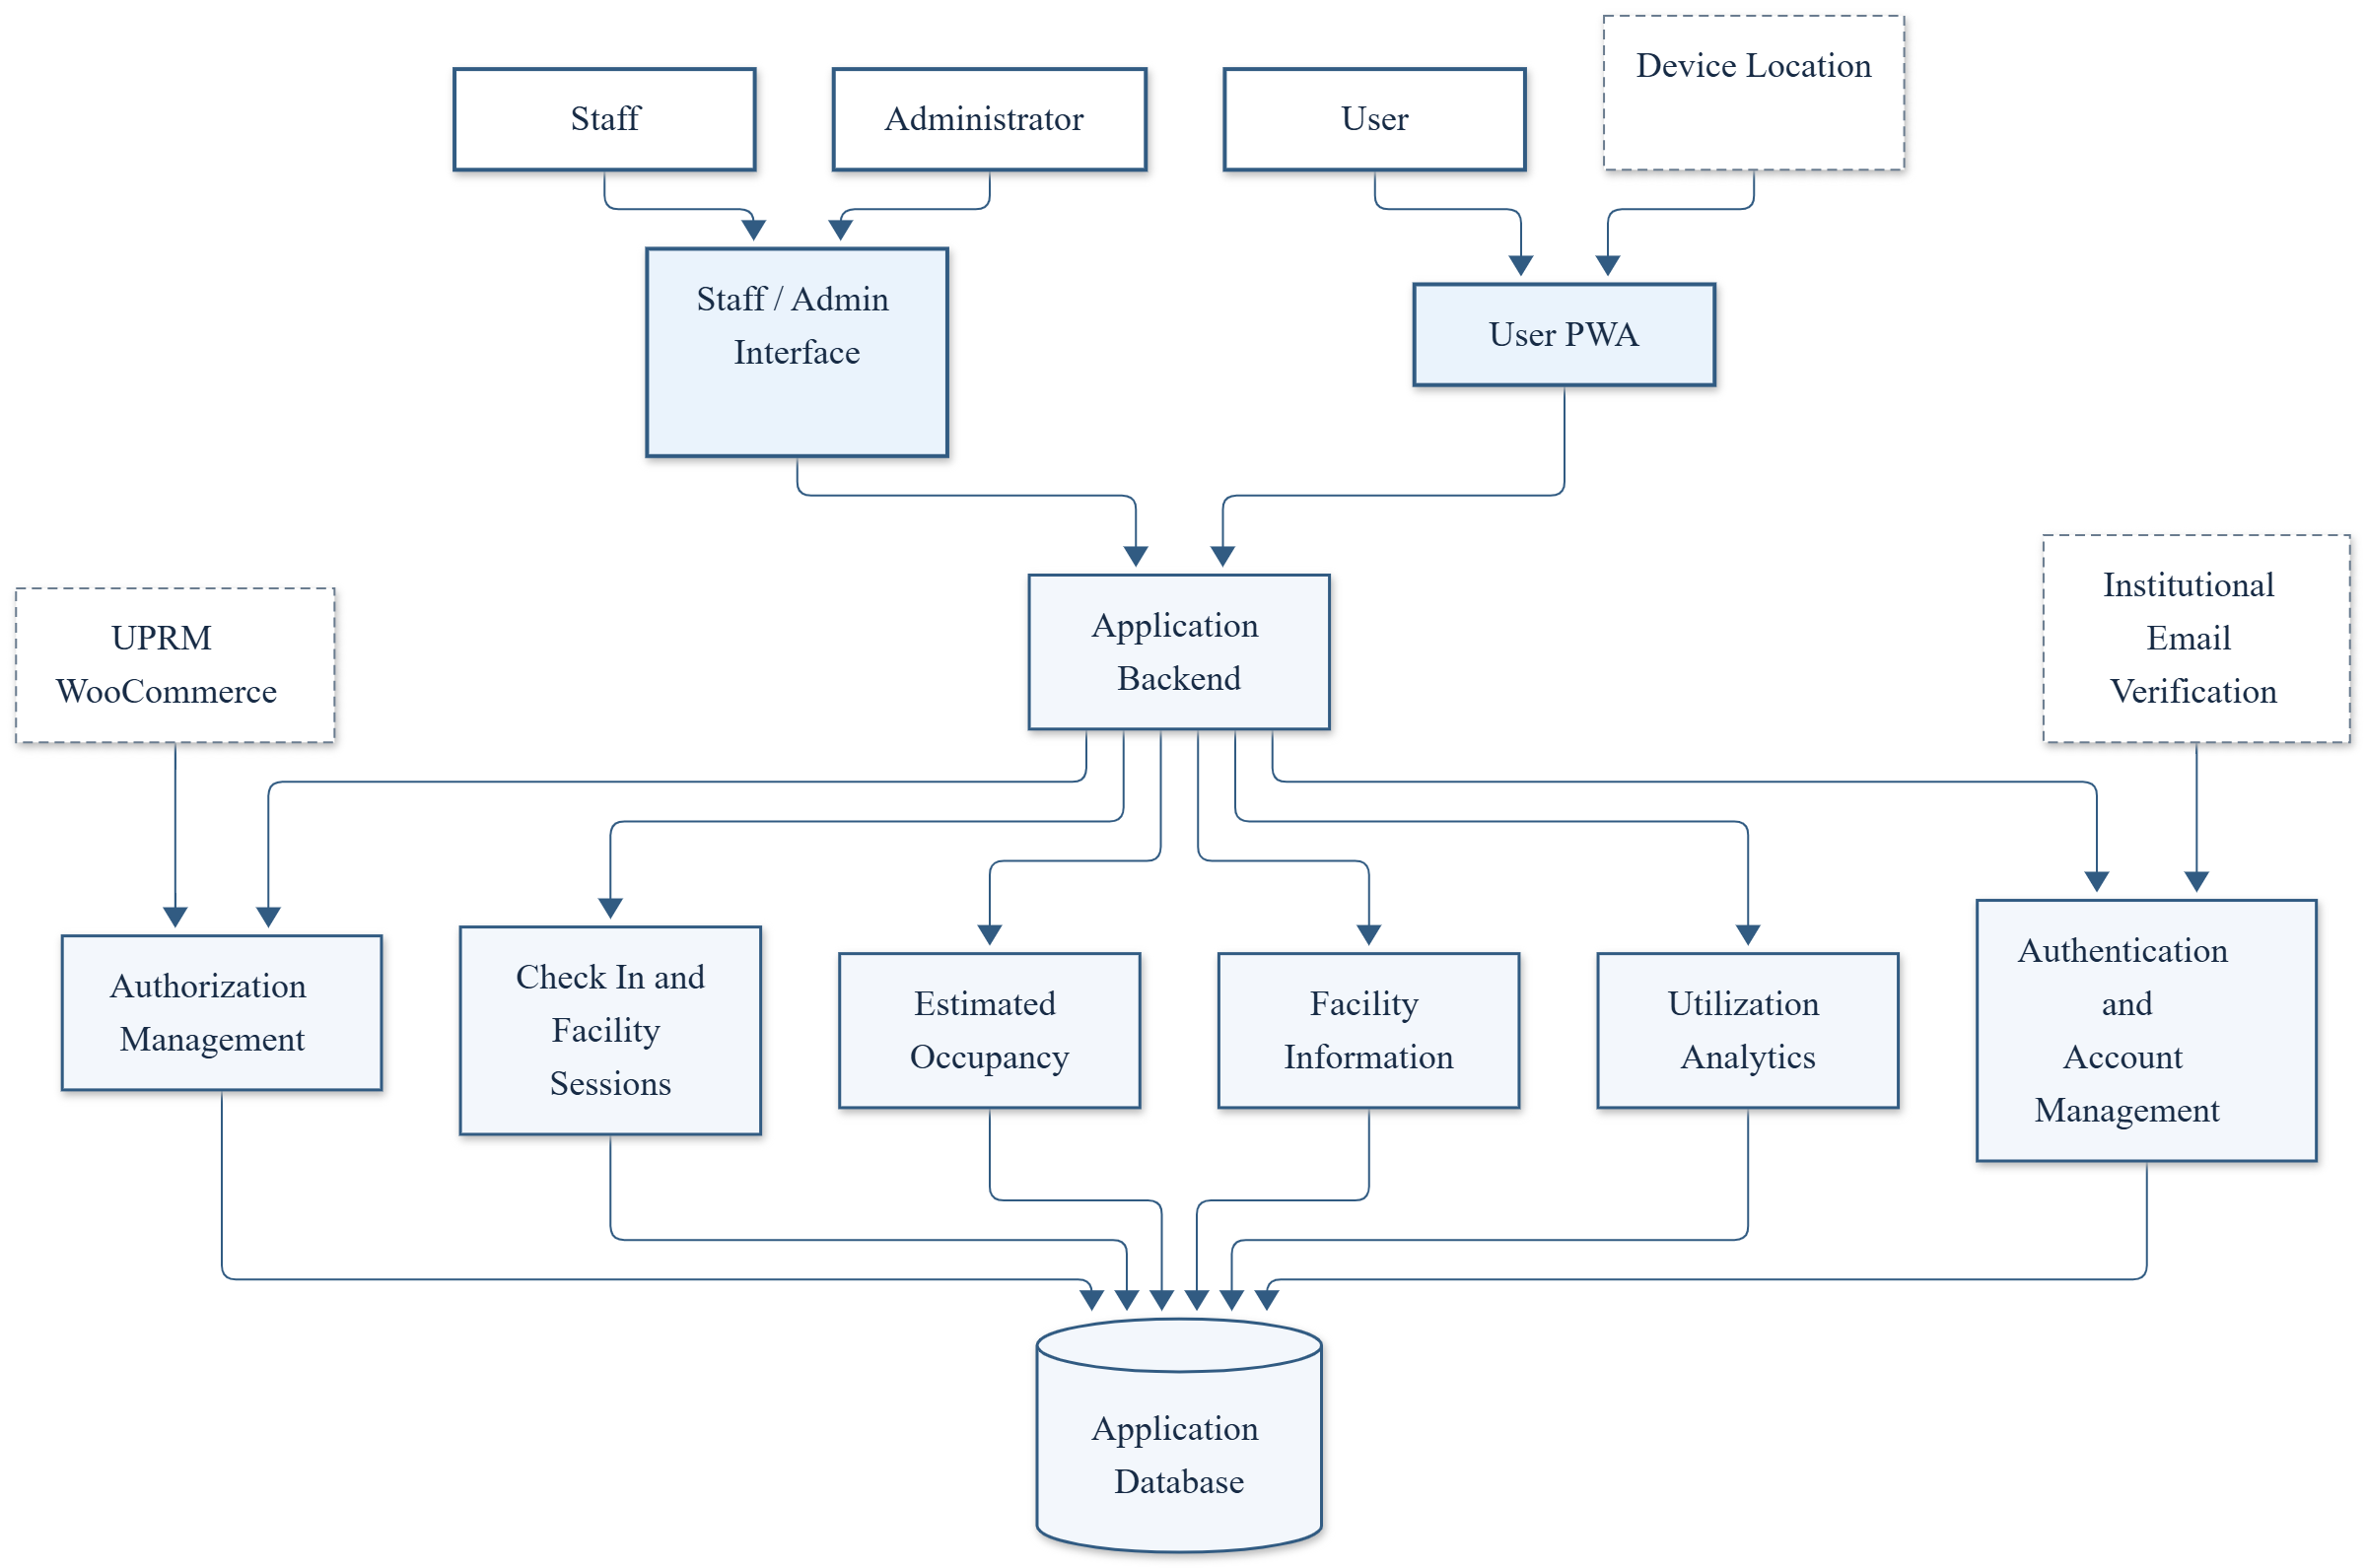
\includegraphics[width=0.9\textwidth,height=0.45\textheight,keepaspectratio]{diagrams/01_architecture.png}
\caption{High-Level System Architecture}
\label{fig:architecture}
\par\vspace{0.35em}\noindent\small\RaggedRight
Figure 1 shows how the User PWA and Staff/Administrator interface connect to the backend, its services, and the application database. WooCommerce, institutional email verification, and device location supply information to the relevant workflows. The figure still shows the proposal's stack. \pending{replace Figure 1 with the container diagram from the architecture document}
\end{figure}

% --------------------------- FIGURE 2 ------------------------------
\begin{figure}[!htbp]
\centering
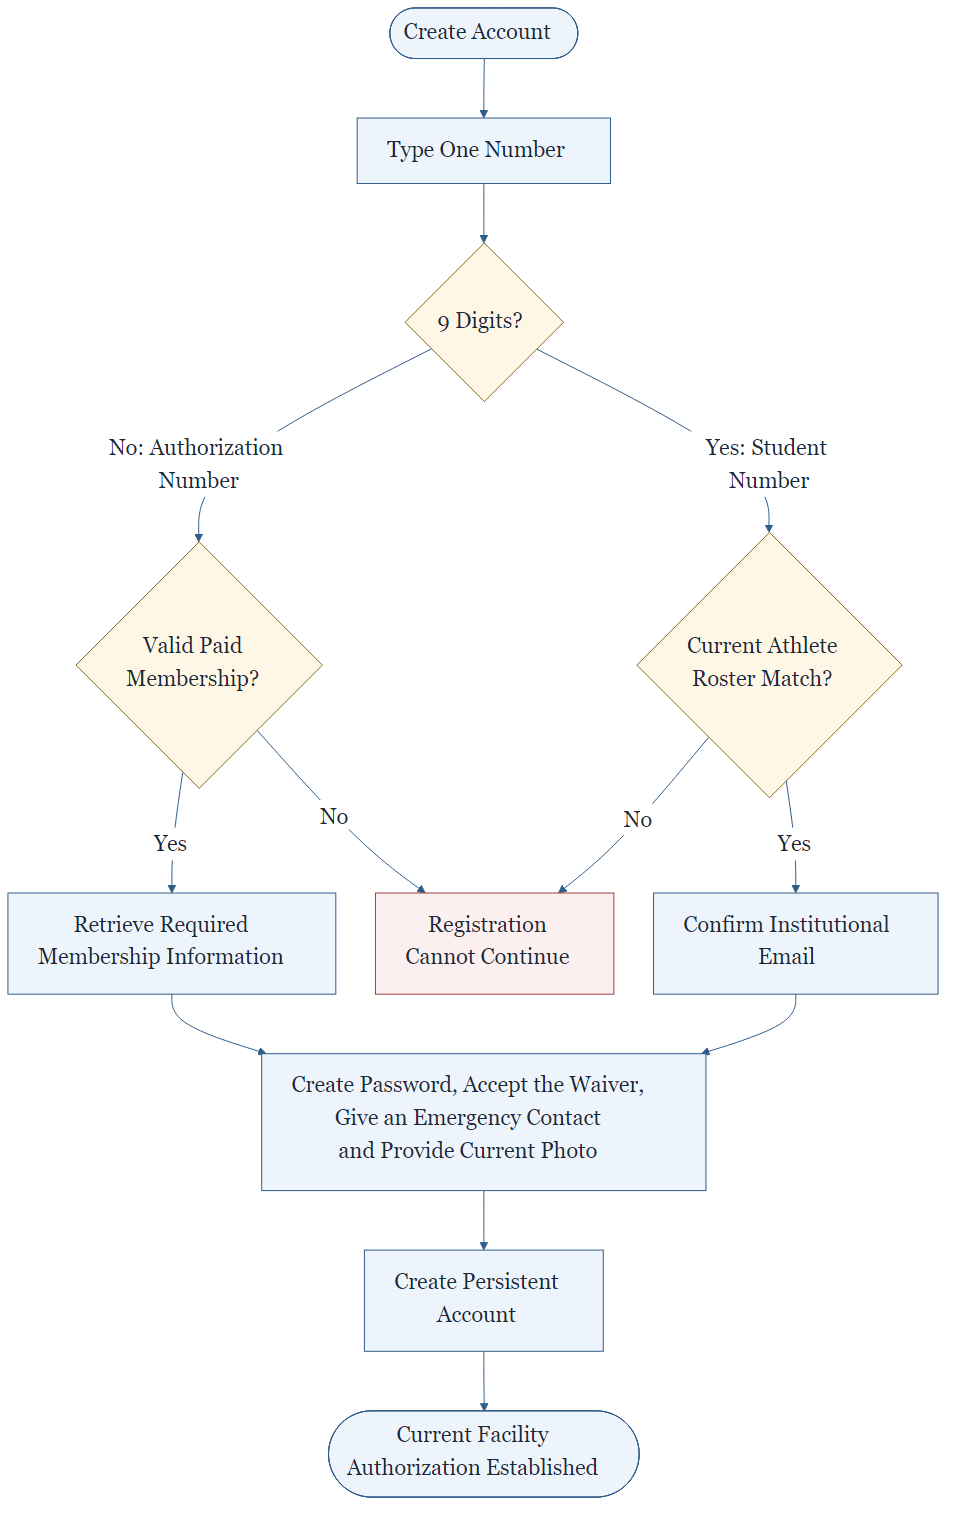
\includegraphics[width=0.98\textwidth,height=0.6\textheight,keepaspectratio]{diagrams/02_account_creation.png}
\caption{Paid-Member and Athlete Account Creation}
\label{fig:accountcreation}
\par\vspace{0.35em}\noindent\small\RaggedRight
Figure 2 separates paid-member validation by Authorization Number from athlete validation against the current roster. Both paths then create one persistent account with a password and current photo. \pending{refresh Figure 2: the Authorization Number lookup limits, the emailed link that creates an athlete account, the photo saved together with the account, and the Staff one-time code}
\end{figure}

% --------------------------- FIGURE 3 ------------------------------
\begin{figure}[!htbp]
\centering
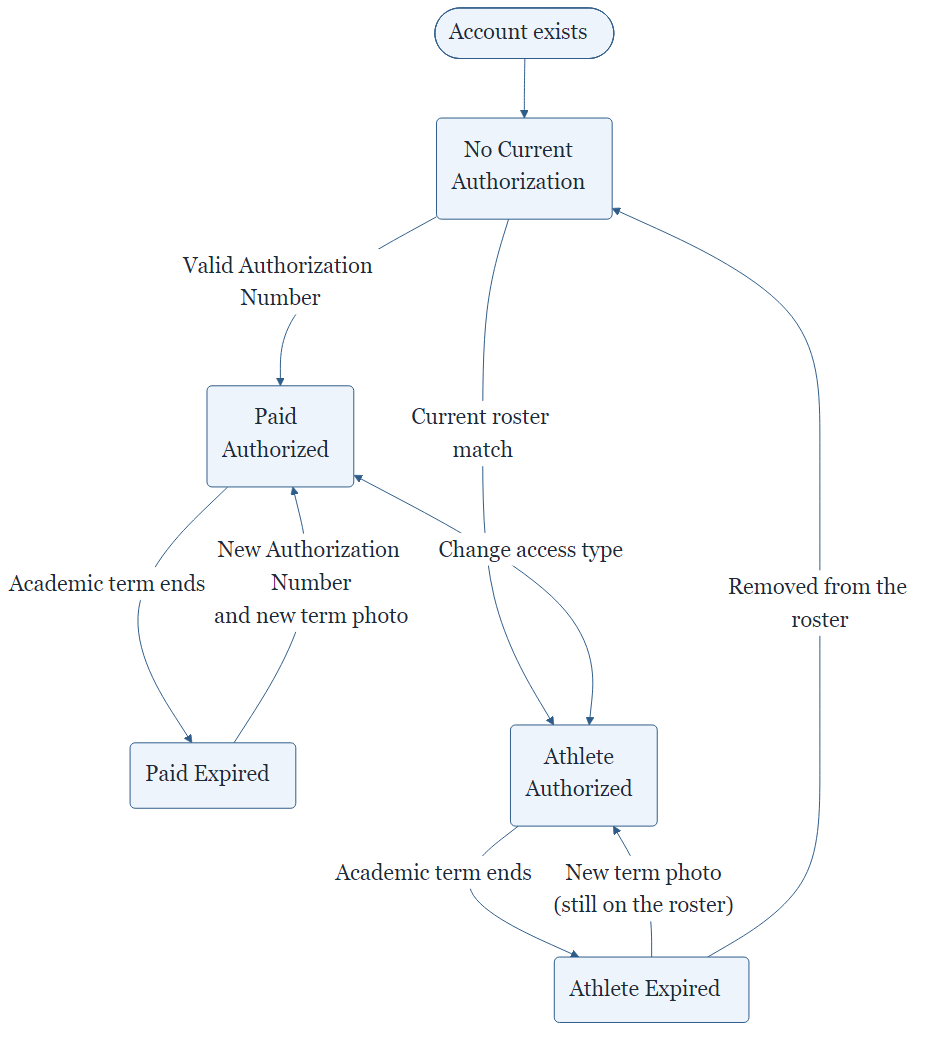
\includegraphics[width=0.98\textwidth,height=0.3\textheight,keepaspectratio]{diagrams/03_authorization_lifecycle.png}
\caption{Post-Registration Account and Authorization Lifecycle}
\label{fig:lifecycle}
\par\vspace{0.35em}\noindent\small\RaggedRight
Figure 3 begins after a persistent account has been established. Authorization may expire, be renewed, or change between paid-member and athlete access while the same User account remains intact. \pending{refresh Figure 3: renewal inside the same account with a new Authorization Number, the ``I am an athlete'' link, the new-term photo, manual grant and revoke, release of a mistaken claim, and import undo}
\end{figure}

% --------------------------- FIGURE 4 ------------------------------
\begin{figure}[!htbp]
\centering
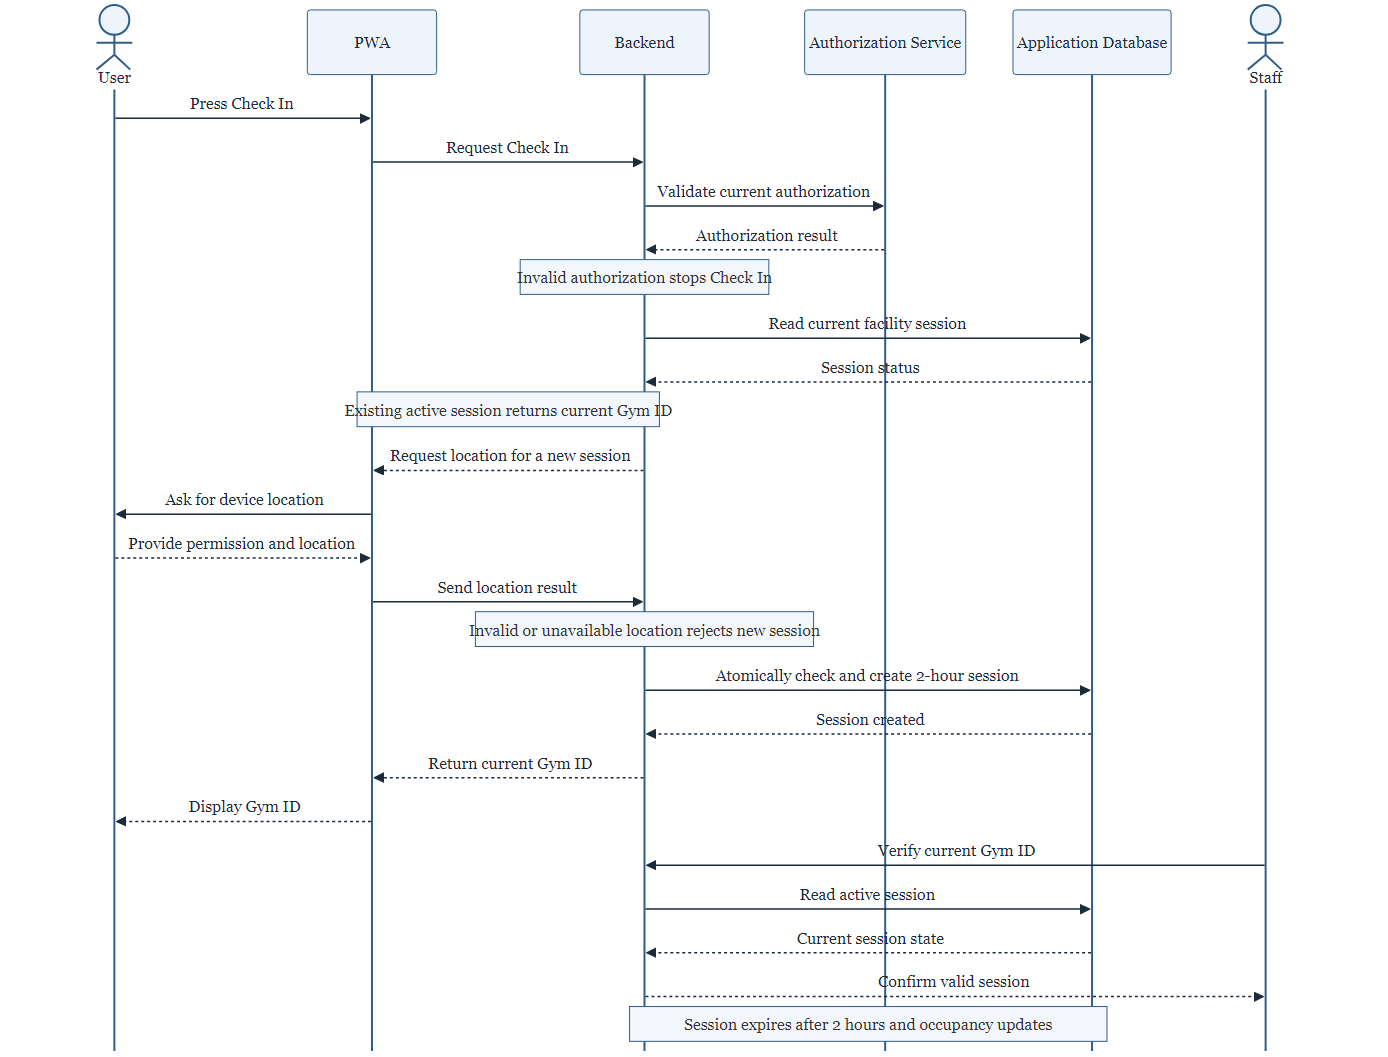
\includegraphics[width=0.98\textwidth,height=0.5\textheight,keepaspectratio]{diagrams/04_checkin_session.png}
\caption{Check-In and Facility Session Sequence}
\label{fig:checkin}
\par\vspace{0.35em}\noindent\small\RaggedRight
Figure 4 shows how authorization, location, active-session control, Gym ID, and Staff verification interact during Check In. The active-session check and session creation are one protected backend operation, so simultaneous requests cannot create overlapping sessions. Location is requested only when a new session is needed. \pending{refresh Figure 4: remove the separate Authorization Service (checks run inside the Laravel app), show the two-step flow with an eligibility query before the Check In request, the cause codes, and the database exclusion constraint}
\end{figure}

% --------------------------- FIGURE 5 ------------------------------
\begin{figure}[!htbp]
\centering
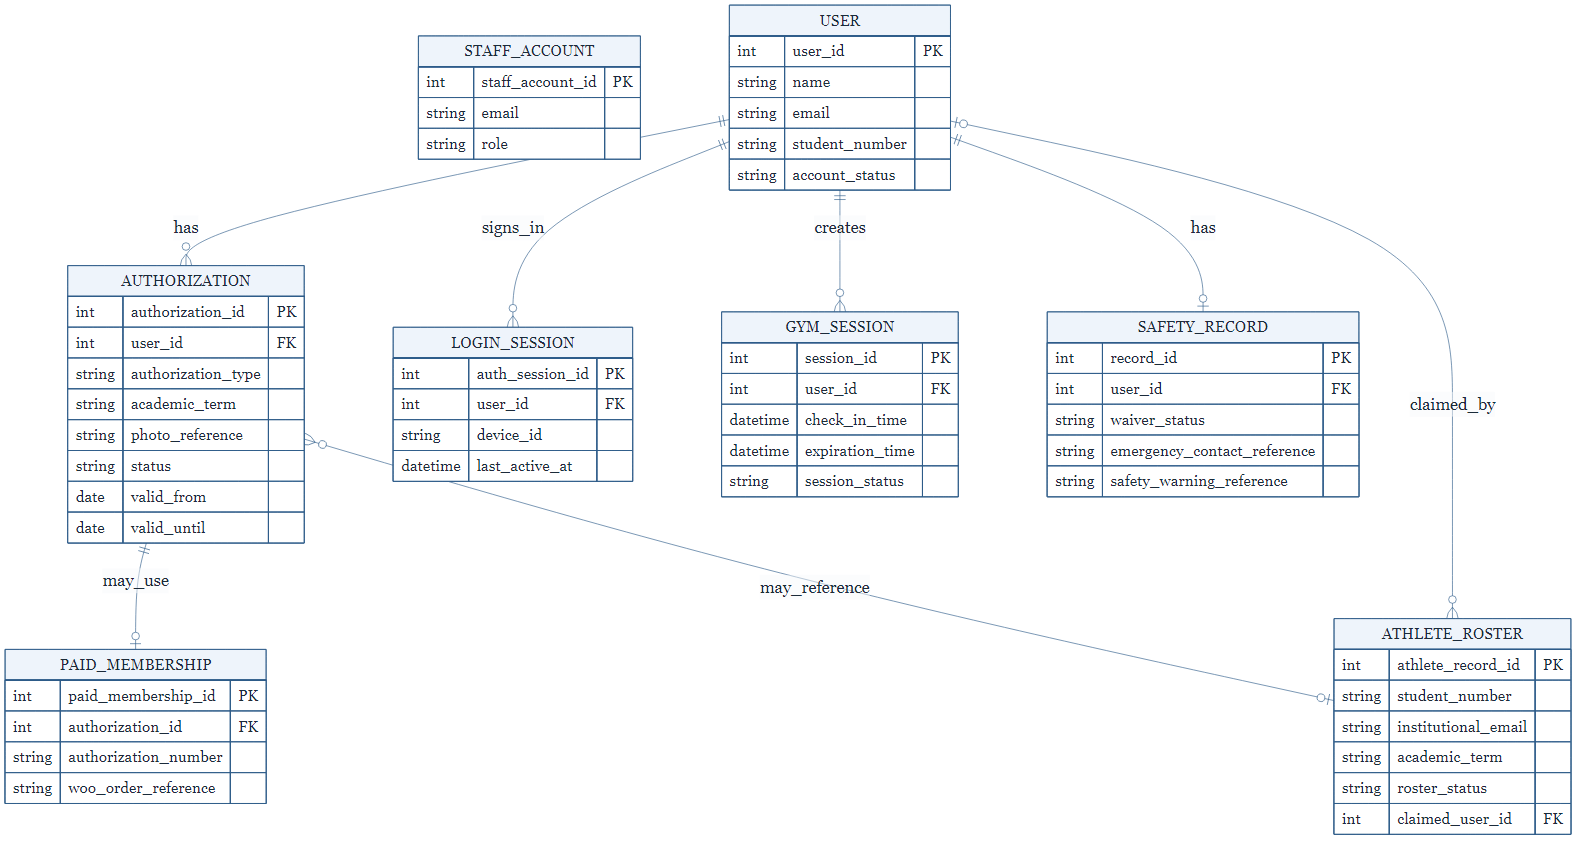
\includegraphics[width=0.98\textwidth,height=0.45\textheight,keepaspectratio]{diagrams/05_data_model.png}
\caption{Conceptual Data Model}
\label{fig:datamodel}
\par\vspace{0.35em}\noindent\small\RaggedRight
Figure 5 separates identity, authorization, sign-in state, facility sessions, roles, and protected membership information. The model keeps semester-specific photographs with Authorization rather than treating the photograph as a permanent User attribute. \pending{refresh Figure 5: add academic terms, imports, imported memberships, roster records, email links, and audit log entries; rename login session to sign-in session; reduce safety records to the waiver acceptance with an emergency contact}
\end{figure}

\subsection{Related Works}

\textbf{Progressive Web Applications.} Królikowski and Miłosz studied factors that affect PWA performance on mobile devices, including resource minimization, lazy loading, and distributed content delivery. The team uses their findings as performance guidance for the PWA [3].

\textbf{Indoor smartphone location.} NIST evaluated smartphone location technologies across five large buildings and found measurable differences in indoor localization performance between Android and iPhone. This supports treating device location as supporting evidence for Check In rather than exact proof of presence, and supports setting the final location boundary and accepted accuracy through tests at the actual Weight Gym [4].

\textbf{Role-Based Access Control.} The NIST RBAC model describes authorization in terms of users, roles, and permissions rather than direct access to every resource. It informs the separation of User, Staff, and Administrator privileges and supports keeping Developer/Maintainer access outside normal gym operational roles [5].

These works shape three engineering decisions: PWA performance, the treatment of indoor device location, and the access-control structure.

\subsection{Engineering Constraints and Verification}

\begin{center}
\small
\begin{longtable}{L{3.1cm} L{5.1cm} L{5.2cm}}
\toprule
\textbf{Constraint and reason} & \textbf{Engineering response} & \textbf{Pass condition / timing} \\
\midrule
\endfirsthead
\toprule
\textbf{Constraint and reason} & \textbf{Engineering response} & \textbf{Pass condition / timing} \\
\midrule
\endhead
\bottomrule
\endlastfoot
\textbf{WooCommerce source.} Membership data remains in an external system. & Keep WooCommerce authoritative, copy only needed fields, and load it from an uploaded Export Orders file so upstream changes do not redesign accounts. & Re-importing a corrected file produces no duplicate, and undo removes what the import brought (Phase 4). \\
\addlinespace
\textbf{Indoor location [4].} Phone accuracy varies by device and indoors. & Require a reading; compare gym boundary and reported accuracy; set the threshold through on-site tests. & Inside, outside, denied-permission, and low-accuracy cases pass on real phones at the gym (Phase 3). \\
\addlinespace
\textbf{Connectivity and polling.} Sign-in, authorization, sessions, one-device enforcement, and Gym ID verification need the backend, and occupancy refreshes by polling every 20 to 30 seconds. & Require connectivity; disable offline Check In to avoid inconsistent access and occupancy; never cache API responses in the service worker. & Offline Sign In and Check In create no session; every screen shows the same occupancy value after its next poll (Phases 3 to 4). \\
\addlinespace
\textbf{Concurrency.} Simultaneous requests can duplicate sessions or claims. & Enforce database uniqueness and exclusion constraints and atomic Check In, not frontend-only checks. & Concurrent requests and repeated Authorization Number or athlete-record claims yield one session or claim; a load test above the expected peak keeps occupancy correct (Phases 3 to 6). \pending{expected peak number from the gym} \\
\addlinespace
\textbf{Browser/device variation.} PWA and geolocation behavior vary. & Test real phones on iPhone/Safari and Android/Chrome; test Windows/Chrome and Edge, with secondary macOS/Firefox checks. & Core flows pass the defined device/browser matrix (Phases 3 to 6). \\
\addlinespace
\textbf{Accessibility.} Users, Staff, and Administrators may use a keyboard, a screen reader, zoom, or a small screen. WCAG 2.2 level AA is required (REQ-NF-13, REQ-NF-14, REQ-NF-36) [6]. & Show states with text or an icon, not color alone; change the page language with the texts; keep tap targets at least 24 by 24 pixels. Verify with axe-core run through Playwright in CI, oxlint jsx-a11y rules, and a manual checklist: keyboard only, NVDA, VoiceOver, 200\% zoom, and a 320 pixel width. & No axe violations on any screen in CI, and the manual checklist passes on the main flows (issue \#82). \\
\addlinespace
\textbf{Sensitive data.} Photos, waivers, emergency contacts, and the audit log need protection. & Restrict by role with Laravel policies, use a private photo volume and minimal collection, and define retention; Staff see only Check In essentials. & Role-permission tests confirm least-needed record access (Phase 5). \\
\addlinespace
\textbf{Mail dependency.} Invitations, athlete links, and password resets need outgoing mail. & Send mail during the request. Use a fake mail server in development and the CTI mail gateway in production, with an external provider only if CTI declines and approves it. & Each link flow works end to end against the fake mail server in tests. \pending{CTI authorization of the VM on its mail gateway} \\
\addlinespace
\textbf{CTI VM.} CTI creates the VM and the domain, but does not manage or maintain the server or the application. & Run the same \texttt{docker-compose} file as in development, with pinned images, and agree a backup and restore procedure with the project owner. & The full stack starts from \texttt{docker-compose} on the VM, and a restore from backup works before the release (Phase 6). \pending{backup method and VM operating system from CTI} \\
\end{longtable}
\end{center}

\subsection{Engineering Standards}

Each standard below applies to a specific technology or risk of the platform.

\begin{center}
\small
\begin{longtable}{L{3.6cm} L{4.4cm} L{5.6cm}}
\toprule
\textbf{Standard} & \textbf{Application to the Project} & \textbf{Justification} \\
\midrule
\endfirsthead
\toprule
\textbf{Standard} & \textbf{Application to the Project} & \textbf{Justification} \\
\midrule
\endhead
\bottomrule
\endlastfoot

WCAG 2.2, relevant Level AA criteria [6]
&
User, Staff, and Administrator web interfaces
&
Targets accessible forms, navigation, touch interactions, and status information. Key states such as the live Gym ID use text or icons in addition to color. Checked by axe-core in CI, lint rules, and a manual checklist. \\
\addlinespace
\midrule
\addlinespace

W3C Geolocation specification [7]
&
Location-based Check In
&
Uses browser-provided geolocation through the standard API. Permission state and reported accuracy are handled in the Check In flow. \\
\addlinespace
\midrule
\addlinespace

NIST SP 800-63B-4, Digital Identity Guidelines: Authentication [8]
&
Passwords, password reset, and sign-in sessions for all accounts
&
Accepts at least 64 characters, sets no composition rules, rejects known breached passwords, limits failed attempts, and answers a reset request the same way for every email. The 10-character minimum deviates from the 15 the standard asks for passwords used alone, because people type on phones. \\
\addlinespace
\midrule
\addlinespace

OWASP ASVS 5.0.0 [9]
&
Authentication, session, and access-control design
&
Consulted for the controls above: hashed passwords, cookie sessions on one origin, per-account and per-IP attempt limits, one device per User, role checks on the server, and an audit log that names the person. \pending{control-by-control mapping and target ASVS level} \\
\addlinespace
\midrule
\addlinespace

NIST RBAC model [5]
&
User, Staff, and Administrator roles
&
Each action is allowed by role through Laravel policies rather than by direct access to a resource. \\
\end{longtable}
\end{center}

\subsection{Engineering Best Practices}

\textbf{Security and access.} Users receive only role-required access, and Staff have no unrestricted administrative access. Developers do not routinely access production safety or emergency data. Laravel policies check every role-restricted action on the server, and the database constraints below back them. Credentials stay in protected server configuration, never in the repository.

\textbf{Integrity and privacy.} Database constraints prevent duplicate athlete-roster and Authorization Number claims and overlapping active sessions. Only needed WooCommerce fields are copied. Location is used for Check In and is not stored as movement history. Photographs use a private volume, and older photographs are discarded unless UPRM requires retention.

\textbf{Reliability and recovery.} WooCommerce data is validated before granting access, and unverifiable records fail safely. Staff corrections, roster changes, imports, and account changes record who acted, what changed, and when. Code and schema stay in Git, and the backup and restore procedure is agreed with the project owner.

\textbf{Development and testing.} Work happens on branches, and a pull request reviewed by another member is required to reach \texttt{main}. GitHub Actions runs on every pull request: lint, unit and database tests, a production build, and a browser test against the full stack started with \texttt{docker-compose}. One \texttt{docker-compose} file gives every member and the CTI VM the same environment, and migrations make the schema reproducible. Planned automated tests will cover authorization and sessions, integration tests will cover sign-in through session creation, and real phones will verify location and PWA behavior. Each Testing Plan case maps to a measurable objective.

%=====================================================================

\section{Project Plan}
%=====================================================================

\subsection{Activities and Process}

\revised{The team follows an iterative process in six phases of one to two weeks each (see the timetable). Each phase ends with a deliverable that someone can check, and the plan lives in a GitHub issue that every member can read. Two milestones, Midterm report (Nov 9) and Final report (Dec 11), group the issues of the phases that end before each date.}

Every piece of work is one GitHub issue. The issue belongs to a milestone and to the Capstone project board, which holds its start and target dates. An issue is sized for one person and about one week: larger work is split, and work under a day joins a related issue. Each issue ends with a ``Done when'' list that a second person can check, and one line of requirement IDs so the work traces back to the SRS.

Each issue gets its own branch, and nothing is committed to \texttt{main} directly. Changes enter through one pull request that links its issue. At least one member besides the author reviews the pull request before it merges. Documents follow the same path as code.

Members pick the issues they want, except setup issues that other work depends on, which go first. After the meetings with CTI and with the Athletic Activities department, the team held standups where decisions were made. Meeting summaries and decisions are posted as announcements in the repository's Discussions with their dates. \revised{When a decision changes the plan, the team updates the plan issue, the affected issues, and the Testing Plan.}

\subsection{Timetable, Milestones, and Deliverables}

\begin{center}
\small
\begin{longtable}{L{1.3cm} L{2.4cm} L{11.3cm}}
\toprule
\textbf{Phase} & \textbf{Dates} & \textbf{Deliverable at the end of the phase} \\
\midrule
\endfirsthead
\toprule
\textbf{Phase} & \textbf{Dates} & \textbf{Deliverable at the end of the phase} \\
\midrule
\endhead
\bottomrule
\endlastfoot
1 & Oct 14 to Oct 25 & Decisions and screens: the team agreed on every open design decision and every screen has an approved wireframe. \\
\addlinespace
2 & Oct 19 to Nov 1 & Foundation: one command starts everything, the PWA opens on a phone, the database exists, and a person can sign in in Spanish or English. \\
\addlinespace
3 & Nov 2 to Nov 8 & Check In: a person with an authorization does Check In inside the gym, sees the Gym ID, and sees the estimated occupancy. An Administrator creates terms and the athlete roster. \textbf{Midterm report, Nov 9.} \\
\addlinespace
4 & Nov 9 to Nov 22 & Registration and sync: people register as paid members or athletes, renew, and become athletes inside their account, and the app reads paid orders from the store. \\
\addlinespace
5 & Nov 16 to Nov 29 & Staff and administration: Staff see active sessions, verify Gym IDs, and do assisted Check In; Administrators manage access, schedules, and notices; everyone sees analytics. \\
\addlinespace
6 & Nov 30 to Dec 11 & Release: the app runs on the CTI server and the gym accepted it. \textbf{Final report, Dec 11.} \\
\end{longtable}
\end{center}

\subsection{Team Responsibilities}

\revised{Each member owns work areas and reviews the others' pull requests. All three met with CTI and the gym and wrote this report. Table~\ref{tab:team} lists what each member did and owns.}

\begin{table}[h]
\centering
\caption{\revised{Work done and owned by each member}}
\label{tab:team}
\small
\begin{tabularx}{\textwidth}{L{3.2cm} X}
\toprule
\textbf{Member} & \textbf{Work done and owned} \\
\midrule
\revised{Carlos J. Pepin Delgado} & \revised{Software Requirements Specification and design documents: architecture, data model, registration, Check In and administration flows, and the screen map by role. Team rules, issue templates, and the wireframe guide. Frontend base and its CI. User app base: phone layout, navigation, install help, and offline support. User sign in on one device, password reset, and account deletion. Check In with location. Gym ID and occupancy. Paid member and athlete registration. Test data for Objective 1 and the load test, with Pierre. Automatic accessibility checks and the flow tests. Project home page. Server requests to CTI.} \\
\addlinespace
\revised{Pierre G. Vales Torres} & \revised{Containers, database, Laravel API, and backend CI. Database tables and rules, and the fake test data. Staff and Administrator accounts: sign in, roles, invitations, password reset, and the audit log. Dashboard base: layout, menu, design tokens, and Spanish and English texts. Staff check-out and the automatic 2-hour close. Academic terms and the athlete roster, with the Word and PDF download. Staff panel: who is inside, assisted Check In, and visit corrections. Occupancy on the dashboard. Security updates and the review of merged pull requests.} \\
\addlinespace
\revised{Viviana V. Ramos Vivoni} & \revised{Wireframes in Figma for registration, Check In and Gym ID, sign in and account, and Staff screens; content, analytics, and administration screens are in progress. The open design decisions of the screen map. User app screens with Carlos: sign in, Gym ID, paid registration, emergency contact, and My visits. Manual accessibility check. Project website on GitHub Pages and the design document updates.} \\
\bottomrule
\end{tabularx}
\end{table}

\subsection{Testing Plan}

Each test belongs to one objective and to one or more requirement IDs (REQ-NF-44), and every case uses a controlled dataset. One seed command loads the same fake data into a fresh local database, and the automated tests and the live demo both run on it, so the demo shows the cases the tests prove.

\revised{\textbf{Unit and regression tests.} Unit tests check each part alone: Vitest for each screen, its states, and the shared code, and PHPUnit for each API route and database rule on PostgreSQL. Playwright browser tests [12] run each flow on the full stack. Continuous integration runs all of them on every pull request and every push to \texttt{main}, so each change reruns the tests of earlier work. The backend workflow also runs lint, migrations, seeding, a health check, and a check that the API answers 503 when the database is down.}

\textbf{Authorization (Phases 3 and 4):} a controlled dataset checks valid and expired paid memberships, valid and invalid athlete approvals, missing authorization, and unmatched users against expected approve and deny decisions. \textbf{Check In and sessions (Phase 3):} tests cover location inside and outside the boundary, denied permission, inadequate accuracy, successful, rejected, and duplicate Check Ins, Staff check-out, the automatic close after 2 hours, closures, and concurrent requests that must create at most one session. Staff-assisted Check In tests (Phase 5) verify the authorized user without a smartphone, photo and authorization checks, actor and timestamp audit, and no overlapping session.

\textbf{Occupancy (Phase 3):} expected active-session counts are compared after Check Ins, check-outs, automatic closes, Staff corrections, and concurrent events; User, Staff, and Administrator views must agree. \textbf{Roles (Phase 5):} the permission matrix confirms allowed actions succeed and forbidden actions fail. \textbf{Analytics (Phase 5):} each finalized metric is compared with a known result from controlled historical data. \textbf{Integration (Phase 6):} one integrated dataset runs from sign in to session creation to analytics, and all five areas are checked together. Engineering-constraint pass conditions and timing appear in Engineering Constraints and Verification.

\revised{\textbf{Concurrency (REQ-NF-42).} A backend test sends simultaneous Check Ins for one user, and repeated Authorization Number or roster claims, to the real database. It passes only with one session or one claim. The load tool cannot release all requests at the same instant, so this check is its own test.}

\revised{\textbf{Accessibility.} An axe-core scan [13] with the WCAG 2.0, 2.1, and 2.2 A and AA rules runs on each screen inside the browser tests and fails the build on a violation, and the linter's accessibility rules are on. A manual checklist covers what a scan cannot: keyboard only, visible focus never covered by the bottom bar, NVDA on Windows, VoiceOver on iPhone, 200\% zoom, a 320 pixel wide screen, and status messages read aloud. Each pull request that adds a screen includes the filled checklist. Scans find only part of the problems, so results claim no automatically detectable violations plus the manual checks, not full WCAG conformance.}

\revised{\textbf{Stress testing with k6 (REQ-NF-15, REQ-NF-42, REQ-NF-50).} k6 scripts [11] sign in the fake users before the timed part and then run three profiles. The gym gave no count for its busiest hour, so the team set the sizes from the estimate of about 150 visits a day: a peak of 50 Check Ins spread over 5 minutes (about a third of the daily visits in the busiest hour, compressed), a stress run of 100 over 5 minutes, and a burst of 50 members at once, each sending two Check Ins in parallel. In the peak and stress runs each member repeats the Check In 60 seconds later and must get the same session. A run passes with a Check In p95 under 3 seconds, errors under 1\%, and every check passing; after the run, the test counts sessions per user and reads the occupancy number. A preliminary run uses the local containers, where k6 and the app share one computer, so its numbers only compare runs with each other. The full run is on the CTI VM. Separately, the Check In button must be usable in under 3 seconds on mobile data on a mid-range phone (REQ-NF-16), which needs a real phone; the test phone and network are \pending{chosen by the team; all three members can test on iPhone and Android}.}

\revised{\textbf{Acceptance testing.} After the release is on the CTI VM, gym staff and real users, both paid members and athletes, run the main flows on their own phones and computers: registration, Check In, Gym ID, Staff-assisted Check In, check-out, and the store sync. Browsers: iPhone with Safari, Android with Chrome, and Windows with Chrome and Edge, with macOS and Firefox as a secondary check (REQ-NF-30, REQ-NF-43, REQ-NF-49). The gym records accepted or not accepted for each flow and the problems found, and each problem becomes an issue. Who takes part and when: \pending{participants and dates, waiting on the gym}.}

%=====================================================================

%=====================================================================
\section{Preliminary Results}
%=====================================================================

\subsection{Performance Results and Documentation}
\pending{8(a): measured numbers with method against targets (load test \#83, CI times, location accuracy at the gym \#12).}

\subsection{Operational Demonstration}
\pending{8(b): working slice of Objectives 1 to 3 on the seeded data (\#81), with screenshots.}

\subsection{Testing Plan Execution}
\pending{8(c): test to objective to requirement table and CI results (\#81), accessibility results (\#82).}

%=====================================================================
\section{\revised{Project Documentation (new)}}
%=====================================================================

\revised{The code is in the repository at \url{https://github.com/Th3-Minorities/natatorio-gym-app}, whose \texttt{README.md} explains how to start the app with one command. The project website at \url{https://th3-minorities.github.io/natatorio-gym-app/} gives the overview, each objective and its status, what is coming, the team, and a guide to the project documents: requirements, design, decisions, meeting summaries, and the submitted proposal.}

\begin{itemize}[leftmargin=1.5em,itemsep=2pt]
\item \revised{\textbf{Issues and board:} every piece of work is a GitHub issue in the Midterm report or Final report milestone and on the Capstone project board of the \texttt{Th3-Minorities} organization.}
\end{itemize}

\section{Previous Work and References}
%=====================================================================

\begingroup\sloppy
\begin{enumerate}[label={[\arabic*]},leftmargin=2.2em,itemsep=6pt]

\item GymMaster, ``All-In-One Gym Management Software.'' [Online]. Available: \url{https://www.gymmaster.com/business/gym-software/}. Accessed: Sep. 29, 2026.

\item TeamUp, ``Access Control Software.'' [Online]. Available: \url{https://goteamup.com/features/access-control}. Accessed: Sep. 29, 2026.

\item Laravel, ``Laravel 13.x Documentation.'' [Online]. Available: \url{https://laravel.com/docs/13.x}. Accessed: Nov. 4, 2026.

\item World Wide Web Consortium (W3C), ``Geolocation.'' [Online]. Available: \url{https://www.w3.org/TR/geolocation/}. Accessed: Sep. 29, 2026.

\item J. Królikowski and M. Miłosz, ``Study of factors affecting the performance of web applications on mobile devices,'' \textit{Journal of Computer Sciences Institute}, vol. 36, pp. 271--277, 2025, doi: 10.35784/jcsi.7430.

\item N. Moayeri, C. Li, and L. Shi, ``Indoor Localization Accuracy of Major Smartphone Location Apps,'' in \textit{Proc. IEEE Wireless Communications and Networking Conference (WCNC)}, Marrakech, Morocco, 2019, doi: 10.1109/WCNC.2019.8885639.

\item R. Sandhu, D. F. Ferraiolo, and D. R. Kuhn, ``The NIST Model for Role-Based Access Control: Towards a Unified Standard,'' in \textit{Proc. Fifth ACM Workshop on Role-Based Access Control}, Berlin, Germany, pp. 47--63, 2000, doi: 10.1145/344287.344301.

\item World Wide Web Consortium (W3C), ``Web Content Accessibility Guidelines (WCAG) 2.2,'' W3C Recommendation, Dec. 12, 2024. [Online]. Available: \url{https://www.w3.org/TR/WCAG22/}. Accessed: Sep. 29, 2026.

\item National Institute of Standards and Technology (NIST), ``Digital Identity Guidelines: Authentication and Authenticator Management,'' NIST SP 800-63B-4. [Online]. Available: \url{https://csrc.nist.gov/pubs/sp/800/63/b/4/final}. Accessed: Nov. 4, 2026.

\item OWASP Foundation, ``OWASP Application Security Verification Standard (ASVS),'' version 5.0.0. [Online]. Available: \url{https://owasp.org/www-project-application-security-verification-standard/}. Accessed: Nov. 4, 2026.

\item Deque Systems, ``axe-core: accessibility engine for automated web UI testing.'' [Online]. Available: \url{https://github.com/dequelabs/axe-core}. Accessed: Nov. 4, 2026.

\item Microsoft, ``Accessibility testing,'' Playwright Documentation. [Online]. Available: \url{https://playwright.dev/docs/accessibility-testing}. Accessed: Nov. 4, 2026.

\item Grafana Labs, ``Grafana k6 Documentation.'' [Online]. Available: \url{https://grafana.com/docs/k6/latest/}. Accessed: Nov. 4, 2026.

\end{enumerate}
\endgroup



\end{document}
